% =====================================================================
%  Exercício Dirigido - Aula 4: caso Caio (app da biblioteca)
%  Design Colaborativo - FEELT31623 - UFU - Prof. Renato Carrijo - 2026/2
%  Compilar com: latexmk -pdf -interaction=nonstopmode ExercicioDirigido_Caio.tex
% =====================================================================
\documentclass[10pt,a4paper]{article}

\usepackage[T1]{fontenc}
\usepackage[utf8]{inputenc}
\IfFileExists{portuges.ldf}{\usepackage[brazil]{babel}}{}
\usepackage[scaled=0.92]{helvet}
\renewcommand{\familydefault}{\sfdefault}
\usepackage{microtype}
\usepackage{amssymb}

\usepackage[a4paper,top=2.2cm,bottom=1.6cm,left=1.8cm,right=1.8cm,headheight=28pt,headsep=10pt]{geometry}
\usepackage[table]{xcolor}
\usepackage{tabularx}
\usepackage{array}
\usepackage{fancyhdr}
\usepackage{enumitem}
\usepackage{fancyvrb}
\usepackage{tikz}
\usetikzlibrary{shapes.geometric,positioning,arrows.meta,calc,fit}
\usepackage[most]{tcolorbox}
\usepackage[hidelinks]{hyperref}
\hypersetup{pdftitle={Exercício Dirigido Aula 4 - Caso Caio},
            pdfauthor={Prisma UX Design}}

% ---------------------------------------------------------------------
%  Paleta (a mesma do relatório + cores das folhas oficiais)
% ---------------------------------------------------------------------
\definecolor{navy}{HTML}{1E3A8A}
\definecolor{navytext}{HTML}{1F2F5C}
\definecolor{bodytext}{HTML}{374151}
\definecolor{labeltext}{HTML}{1F2937}
\definecolor{gridline}{HTML}{9CA3AF}
\definecolor{secbg}{HTML}{E8EDF5}
\definecolor{subtle}{HTML}{4B5563}
\definecolor{cream}{HTML}{FFF8E1}
\definecolor{gold}{HTML}{D4A017}
\definecolor{amber}{HTML}{B45309}
\definecolor{laranja}{HTML}{E67E22}   % golfo de avaliação, ideias, hipóteses
\definecolor{laranjabg}{HTML}{FCEBDD}
\definecolor{verde}{HTML}{0F7B5F}     % usuários, benefícios
\definecolor{verdebg}{HTML}{DDF0EA}
\definecolor{dor}{HTML}{DC2626}       % pontos de dor
\definecolor{cinzabg}{HTML}{ECECEC}

% ---------------------------------------------------------------------
%  Dados da equipe (os mesmos de Entrega_01/UX_final.tex)
% ---------------------------------------------------------------------
\newcommand{\equipenome}{Prisma UX Design}
\newcommand{\dataentrega}{27/10/2026}
\newcommand{\integrantes}{Wilson Ribeiro de Andrade Filho (líder) \textbullet\ José Mendes de Sousa \textbullet\ José Lucas Lira \textbullet\ Ana Flávia de Oliveira \textbullet\ Emanuel Simões Campos}

% ---------------------------------------------------------------------
%  Cabeçalho e rodapé
% ---------------------------------------------------------------------
\pagestyle{fancy}
\fancyhf{}
\fancyhead[L]{\textcolor{navytext}{\bfseries\small DESIGN COLABORATIVO \textbullet\ FEELT31623}}
\fancyhead[R]{\footnotesize\color{subtle}%
  \begin{tabular}[b]{@{}r@{}}Universidade Federal de Uberlândia\\
  Prof. Renato Carrijo \textbullet\ 2026/2\end{tabular}}
\fancyfoot[C]{\footnotesize\color{subtle}\equipenome\ \textbullet\ \thepage}
\renewcommand{\headrulewidth}{0.8pt}
\renewcommand{\headrule}{{\color{navytext}\hrule height\headrulewidth width\headwidth}}

\setlength{\parindent}{0pt}
\setlength{\tabcolsep}{5pt}
\arrayrulecolor{gridline}
\setlist{nosep,leftmargin=1.2em}

% ---------------------------------------------------------------------
%  Macros das folhas
% ---------------------------------------------------------------------
% Faixa azul do título da folha: {título}{tempo}
\newcommand{\folha}[2]{%
  \noindent
  \colorbox{navy}{\parbox{\dimexpr\linewidth-2\fboxsep\relax}{%
    \vspace{3pt}%
    \textcolor{white}{\bfseries\large #1}\hfill
    \ifx&#2&\else\colorbox{laranja}{\textcolor{white}{\bfseries\small #2}}\fi\\[1pt]
    \textcolor{white}{\scriptsize Design Colaborativo -- FEELT31623 -- Aula 4: Exercício Dirigido -- Prof. Renato Carrijo}%
    \vspace{3pt}}}%
  \par\vspace{5pt}
  {\small\textbf{Equipe:} \equipenome\hfill\textbf{Data:} \dataentrega\par}
  {\scriptsize\color{subtle}\textbf{Integrantes:} \integrantes\par}
  \vspace{4pt}}

% Faixa "Objetivo" (creme com borda laranja)
\newcommand{\objetivo}[1]{%
  \begin{tcolorbox}[colback=laranjabg,colframe=laranja,boxrule=0.5pt,arc=0pt,
    left=3pt,right=3pt,top=1pt,bottom=1pt,fontupper=\small]
  \textbf{Objetivo:} #1
  \end{tcolorbox}\vspace{-4pt}}

% Linha de passos
\newcommand{\passos}[1]{{\footnotesize\textbf{Passos:} #1\par}\vspace{4pt}}

% Caixa com título (azul por padrão; cor como argumento opcional)
\newtcolorbox{caixa}[2][navy]{enhanced,colback=white,colframe=#1,colbacktitle=#1,
  coltitle=white,fonttitle=\bfseries\small,title={#2},boxrule=0.6pt,arc=2pt,
  left=4pt,right=4pt,top=3pt,bottom=3pt,fontupper=\small\color{bodytext},
  before skip=4pt,after skip=4pt}

% Rótulo dos movimentos do Gamestorming
\newcommand{\mov}[1]{\colorbox{laranjabg}{\textcolor{amber}{\scriptsize\bfseries #1}}}

% Palavras-chave do Gherkin
\newcommand{\gk}[1]{\textcolor{navy}{\bfseries #1}}

% Bolinha de ponto de dor e de voto
\newcommand{\pdor}{\tikz[baseline=-0.6ex]\node[circle,draw=dor,line width=1pt,inner sep=0.8pt,text=dor,font=\tiny\bfseries]{!};}
\newcommand{\votos}[1]{\tikz[baseline=-0.6ex]{\foreach \i in {1,...,#1}{\fill[navy] (\i*5pt,0) circle (1.8pt);}}}

% Cabeçalhos coloridos da tabela de requisitos
\newcommand{\cab}[2]{\cellcolor{#1}\bfseries\footnotesize #2}

% =====================================================================
\begin{document}

% =====================================================================
%  FICHA DA EQUIPE E DO CASO
% =====================================================================
\folha{Ficha da Equipe e do Caso}{}

{\small
\textbf{Nome da equipe (como o de uma empresa):} \equipenome\par\vspace{2pt}
\textbf{Líder (quem posta a entrega):} Wilson Ribeiro de Andrade Filho\par}
\vspace{6pt}

{\footnotesize\renewcommand{\arraystretch}{1.35}%
\noindent
\begin{tabularx}{\linewidth}{|c|>{\raggedright\arraybackslash}X|c|>{\centering\arraybackslash}p{2.15cm}|>{\centering\arraybackslash}p{2.15cm}|>{\centering\arraybackslash}p{2.15cm}|>{\centering\arraybackslash}p{2.15cm}|}
\hline
\rowcolor{secbg}\bfseries N. & \bfseries Nome do integrante & \bfseries Matrícula & \bfseries Papel inicial\newline(etapas 1--2) & \bfseries Papel (troca)\newline(etapas 3--4) & \bfseries Etapas 5--6 & \bfseries Etapas 7--8 \\ \hline
1 & Wilson Ribeiro de Andrade Filho (líder) & 12311ECP006 & Facilitador & Cronometrista & Relator & Desenhista \\ \hline
2 & José Mendes de Sousa & 12211ECP012 & Cronometrista & Relator & Desenhista & Guardião do usuário \\ \hline
3 & José Lucas Lira & 12411ECP005 & Relator & Desenhista & Guardião do usuário & Facilitador \\ \hline
4 & Ana Flávia de Oliveira & 12411ECP025 & Desenhista & Guardião do usuário & Facilitador & Cronometrista \\ \hline
5 & Emanuel Simões Campos & 12311ECP031 & Guardião do usuário & Facilitador & Cronometrista & Relator \\ \hline
\end{tabularx}\par}
\vspace{2pt}
{\scriptsize\color{subtle}Papéis: Facilitador (conduz), Cronometrista (tempo), Relator (registra), Desenhista (figuras), Guardião do usuário (``a persona entenderia?''). O rodízio anda uma posição a cada duas etapas, então cada pessoa passa por quatro papéis diferentes. A folha oficial pede só ``inicial'' e ``troca'': transcrevam as duas primeiras colunas de papéis.\par}

\begin{caixa}{Caso: aplicativo fictício da biblioteca da faculdade}
\textbf{Persona:} Caio, 19 anos, calouro de Engenharia de Computação. Tem prova na sexta e o livro de Cálculo vence amanhã. Usa o celular no ônibus, com pouca bateria (5\%) e sinal fraco (3G instável).\par\vspace{2pt}
\textbf{O que acontece hoje:} (1) em ``Meus empréstimos'' o botão \textit{Renovar} aparece cinza, sem explicação; (2) há uma multa pendente, mas ela só aparece em outra aba; (3) ao tocar em \textit{Renovar}, nada confirma a nova data; (4) não há aviso antes do vencimento.\par\vspace{2pt}
\textbf{Objetivo do negócio:} reduzir em 30\% as devoluções em atraso. \textbf{Objetivo da persona:} renovar o livro sem ir à biblioteca.
\end{caixa}

{\small\renewcommand{\arraystretch}{1.3}%
\noindent
\begin{tabularx}{\linewidth}{@{}>{\color{navy}}l X r @{\hspace{14pt}} >{\color{navy}}l X r@{}}
\hline
\multicolumn{3}{@{}l}{\bfseries Etapa} & \multicolumn{3}{l@{}}{\bfseries Etapa} \\ \hline
$\boxtimes$ & 1. Modelo mental e golfos & 10 min & $\boxtimes$ & 5. Requisitos & 10 min \\
$\boxtimes$ & 2. Cenário (Gamestorming) & 15 min & $\boxtimes$ & 6. Histórias e critérios & 15 min \\
$\boxtimes$ & 3. Análise hierárquica (HTA) & 10 min & $\boxtimes$ & 7. Features e priorização & 15 min \\
$\boxtimes$ & 4. Fluxo de tarefas & 10 min & $\boxtimes$ & 8. UX Canvas e pitch & 15 min \\ \hline
\end{tabularx}\par}
\vspace{4pt}
{\scriptsize\color{subtle}Regras: em ``abrir'', ninguém critica ideias; uma ideia por post-it; usem o cronômetro; não apaguem folhas antigas. Avaliação total: 10 pontos.\par}

\vspace{8pt}
\begin{caixa}[verde]{Como este documento foi montado}
Cada folha usa o resultado da anterior (golfos $\rightarrow$ cenário $\rightarrow$ HTA $\rightarrow$ fluxo $\rightarrow$ requisitos $\rightarrow$ histórias $\rightarrow$ features $\rightarrow$ canvas). Os códigos se repetem de uma folha para outra para facilitar o rastreio: \textbf{E1--E4} (golfo de execução), \textbf{A1--A4} (golfo de avaliação), \textbf{R1--R4} (requisitos), \textbf{H1--H4} (histórias), \textbf{F1--F9} (features). A solução (Folha 4) leva a renovação para a tela inicial: um toque no card do livro, e o resto o app resolve em segundo plano. Os problemas de cada passo foram justificados com as heurísticas de Nielsen (H.\,1 a H.\,10) e com as leis de ergonomia (Fitts, zona do polegar).
\end{caixa}

\newpage
% =====================================================================
%  FOLHA 1 - MODELO MENTAL E GOLFOS
% =====================================================================
\folha{Folha 1 -- Modelo mental e golfos}{10 min}
\objetivo{Descobrir onde Caio não sabe \textit{como fazer} (golfo de execução) e onde não sabe \textit{se deu certo} (golfo de avaliação).}
\passos{(1) Sozinhos, 3 min: escreva num post-it como você acha que renovar um livro funciona no app. (2) Em grupo, 3 min: comparem e marquem as diferenças. (3) 4 min: listem os golfos do caso, mínimo 2 em cada coluna.}

\begin{caixa}{Diferenças entre os modelos mentais da equipe}
\begin{itemize}
  \item \textbf{Automático $\times$ manual:} parte da equipe achava que o app renova sozinho quando ninguém reservou o livro; a outra parte, que é preciso tocar em \textit{Renovar}.
  \item \textbf{Multa bloqueia?} Uns achavam que a multa só é cobrada na devolução e não impede renovar; outros sabiam que ela trava qualquer empréstimo novo.
  \item \textbf{Onde fica a pendência:} uns esperavam ver a multa junto do livro; outros lembraram que ela fica numa aba separada (``Débitos'').
  \item \textbf{Quando ``está renovado'':} uns achavam que basta tocar no botão; outros, que só vale quando aparece a nova data.
\end{itemize}
\textbf{Conclusão:} o modelo mental mais provável de Caio é ``toco em Renovar e pronto''. O app não corrige essa ideia em nenhum momento.
\end{caixa}

\begin{tcbraster}[raster columns=2,raster equal height,raster column skip=8pt,raster before skip=6pt]
\begin{caixa}{Golfo de execução: ``como eu faço?''}
\begin{enumerate}[label=\textbf{E\arabic*.},leftmargin=2em,itemsep=5pt]
  \item \textbf{Botão cinza sem explicação.} \textit{Renovar} aparece desativado, sem texto nem ícone de motivo. Caio não sabe se está bloqueado, carregando ou com defeito: falta um \textit{signifier} (sinal que diga o que fazer).\newline{\scriptsize\color{subtle}Nielsen H.\,1 (status do sistema) e H.\,9 (ajudar a entender o erro).}
  \item \textbf{Multa escondida em outra aba.} A causa do bloqueio está em ``Débitos'', longe da tela onde Caio está. Ele precisaria lembrar que essa aba existe.\newline{\scriptsize\color{subtle}Nielsen H.\,6 (reconhecer em vez de lembrar).}
  \item \textbf{Sem caminho para pagar.} Mesmo achando a multa, o app não diz como quitá-la nem se dá para pagar por ele: é um beco sem saída.\newline{\scriptsize\color{subtle}Nielsen H.\,9 e H.\,10 (ajuda).}
  \item \textbf{Alvo pequeno, longe do polegar.} No ônibus balançando, com uma mão, o botão pequeno no alto do card é difícil de acertar.\newline{\scriptsize\color{subtle}Lei de Fitts e zona do polegar.}
\end{enumerate}
\end{caixa}
\begin{caixa}[laranja]{Golfo de avaliação: ``deu certo?''}
\begin{enumerate}[label=\textbf{A\arabic*.},leftmargin=2em,itemsep=5pt]
  \item \textbf{Toque sem resposta.} Depois de tocar em \textit{Renovar}, nada muda na tela e a nova data de devolução não aparece.\newline{\scriptsize\color{subtle}Nielsen H.\,1 (status do sistema).}
  \item \textbf{Rede invisível.} Com o 3G caindo, Caio não sabe se o pedido saiu do celular, se está pendente ou se falhou; tende a tocar várias vezes, gastando a pouca bateria.\newline{\scriptsize\color{subtle}Nielsen H.\,1 e H.\,9.}
  \item \textbf{Prazo sem aviso.} Nada avisou que o livro vencia; Caio só percebe na véspera, quando qualquer imprevisto vira atraso.\newline{\scriptsize\color{subtle}Nielsen H.\,1 e H.\,5 (prevenção de erros).}
  \item \textbf{Multa paga $\neq$ livro renovado.} Se Caio pagar a multa, nada indica que a renovação foi liberada nem que precisa tocar de novo.\newline{\scriptsize\color{subtle}Nielsen H.\,1.}
\end{enumerate}
\end{caixa}
\end{tcbraster}

\newpage
% =====================================================================
%  FOLHA 2 - CENÁRIO (GAMESTORMING)
% =====================================================================
\folha{Folha 2 -- Cenário (Gamestorming)}{15 min}
\objetivo{Escrever uma pequena história de uso de Caio, com obstáculo, e extrair requisitos candidatos.}
\passos{(1) Escolher, 2 min. (2) Situar, 3 min: preencha o quadro. (3) Narrar, 6 min: uma ação por post-it, ordenem na parede e escrevam o parágrafo. (4) Provocar, 4 min: sorteiem um obstáculo e reescrevam.}

\begin{caixa}{Situar}
\renewcommand{\arraystretch}{1.35}%
\begin{tabularx}{\linewidth}{@{}>{\bfseries}p{2.2cm}X>{\bfseries}p{1.8cm}X@{}}
Onde: & Em pé, num ônibus lotado a caminho do campus. & Hora: & Terça-feira, 27/10, 7h40 (aula às 8h). \\
Aparelho: & Celular Android de entrada, uma mão livre, 5\% de bateria, 3G instável. & Pressão: & O livro vence amanhã (28/10); prova de Cálculo na sexta (30/10); não dá tempo de ir à biblioteca. \\
Obstáculo: & \multicolumn{3}{X}{Sorteado: ``o sinal cai''. Somado ao do caso: a renovação está bloqueada por uma multa que só aparece em outra aba.} \\
\end{tabularx}
\end{caixa}

\begin{caixa}{Cenário (6 a 8 linhas)}
\setlength{\parskip}{0pt}\linespread{1.25}\selectfont
\mov{ESCOLHER} Caio, 19 anos, calouro de Engenharia de Computação, quer renovar hoje o livro de Cálculo para estudar até a prova de sexta.
\mov{SITUAR} Terça, 7h40, em pé no ônibus, ele abre o app da biblioteca com uma mão e o celular em 5\% de bateria.
\mov{NARRAR} Entra em ``Meus empréstimos'', acha o livro e vê o botão \textit{Renovar} cinza, sem nenhuma explicação. Toca três vezes e nada acontece; desconfia de defeito, fecha e reabre o app, gastando mais bateria.
\mov{PROVOCAR} Na nova tentativa o 3G cai. Quando o sinal volta, Caio descobre por acaso, na aba ``Débitos'', uma multa de R\$\,2,00 de um atraso antigo. Sem saber se pode pagar pelo app nem se o primeiro pedido chegou a ser enviado, ele desiste: o celular apaga, e o livro vence amanhã.
\end{caixa}

\begin{caixa}{Requisitos candidatos (mínimo 3)}
\begin{enumerate}[label=\textbf{RC\arabic*.},leftmargin=2.6em,itemsep=4pt]
  \item Mostrar, no próprio livro, \textbf{por que} a renovação está bloqueada e \textbf{como resolver} (E1, E2).
  \item Permitir \textbf{pagar a multa dentro do app}, a partir do mesmo card, e liberar a renovação logo depois (E3, A4).
  \item \textbf{Confirmar} a renovação com a nova data de devolução, que continue visível mesmo sem internet (A1).
  \item Concluir a renovação \textbf{em segundo plano}: se o sinal cair, reenviar sozinho quando ele voltar, sem pedido duplicado e sem exigir nada do aluno (A2).
  \item \textbf{Avisar antes do vencimento}, com um atalho para renovar (A3).
\end{enumerate}
\end{caixa}

{\scriptsize\color{subtle}Para a folha oficial, basta transcrever os 4 movimentos como um parágrafo corrido; os rótulos laranjas mostram onde cada movimento começa.\par}

\newpage
% =====================================================================
%  FOLHA 3 - HTA
% =====================================================================
\folha{Folha 3 -- Análise hierárquica de tarefas (HTA)}{10 min}
\objetivo{Dividir a tarefa ``Renovar livro'' em subtarefas e ações observáveis e marcar os pontos de dor.}
\passos{(1) Objetivo no topo. (2) 3 a 5 subtarefas. (3) Ações observáveis em cada subtarefa. (4) Escreva o plano 0. (5) Circule em vermelho os pontos de dor.}

\begin{center}
\begin{tikzpicture}[
  font=\footnotesize,
  topo/.style={draw=navy,fill=secbg,rounded corners=2pt,minimum width=5cm,minimum height=0.9cm,font=\normalsize\bfseries,text=navytext},
  sub/.style={draw=navy,fill=white,rounded corners=2pt,text width=3.55cm,minimum height=1.0cm,align=center,font=\footnotesize\bfseries,text=navytext},
  acao/.style={draw=laranja,fill=white,rounded corners=2pt,text width=3.55cm,minimum height=1.25cm,align=center,font=\scriptsize,text=bodytext},
  doracao/.style={acao,draw=dor,line width=1.4pt},
  liga/.style={draw=gridline,line width=0.6pt},
  marca/.style={circle,fill=dor,text=white,inner sep=1pt,font=\tiny\bfseries}
]
  \node[topo] (t0) at (0,0) {0. Renovar livro};
  \foreach \i/\x/\txt in {1/-6.45/Acessar empréstimos, 2/-2.15/Localizar o livro, 3/2.15/Resolver a pendência (multa), 4/6.45/Renovar e confirmar}{
    \node[sub] (s\i) at (\x,-1.8) {\i. \txt};
    \draw[liga] (t0.south) -- ++(0,-0.45) -| (s\i.north);
  }
  % ações (empilhadas sob cada subtarefa)
  \node[acao]    (a11) at (-6.45,-3.45) {\textbf{1.1} Abrir o app (login salvo)};
  \node[acao]    (a12) at (-6.45,-5.0)  {\textbf{1.2} Tocar em ``Meus empréstimos''};
  \node[acao]    (a21) at (-2.15,-3.45) {\textbf{2.1} Achar ``Cálculo I'' e ver o vencimento (28/10)};
  \node[doracao] (a22) at (-2.15,-5.0)  {\textbf{2.2} Ver se \textit{Renovar} está ativo\\(hoje: cinza, sem motivo)};
  \node[doracao] (a31) at (2.15,-3.45)  {\textbf{3.1} Descobrir o motivo\\do bloqueio\\(hoje: só na aba ``Débitos'')};
  \node[doracao] (a32) at (2.15,-5.0)   {\textbf{3.2} Pagar a multa de R\$\,2,00\\(hoje: app não diz como)};
  \node[doracao] (a41) at (6.45,-3.45)  {\textbf{4.1} Tocar em \textit{Renovar}\\(3G instável, sem retorno)};
  \node[doracao] (a42) at (6.45,-5.0)   {\textbf{4.2} Conferir a nova data\\(hoje: não aparece)};
  \foreach \s in {1,2,3,4}{
    \draw[liga] (s\s.south) -- (a\s1.north);
    \draw[liga] (a\s1.south) -- (a\s2.north);
  }
  \foreach \n in {a22,a31,a32,a41,a42}{\node[marca] at (\n.north east) {!};}
  % legenda
  \node[draw=dor,line width=1.4pt,rounded corners=2pt,minimum width=0.6cm,minimum height=0.35cm] (leg) at (-6.9,-6.15) {};
  \node[anchor=west,font=\scriptsize,text=subtle] at (leg.east) {= ponto de dor (circulado em vermelho na folha)};
\end{tikzpicture}
\end{center}
\vspace{-2pt}

\begin{caixa}{Plano 0 (ordem, escolha ou repetição)}
\textbf{Plano 0:} faça 1 e depois 2. \textbf{Se} em 2.2 o botão estiver ativo, vá direto para 4. \textbf{Se} estiver inativo por multa, faça 3 (3.1 e depois 3.2) e repita 2.2 antes de 4. Em 4.1, \textbf{se} não houver resposta em 10 s, repita 4.1 (até 3 vezes) ou deixe o pedido na fila até o sinal voltar. \textbf{Termine} quando 4.2 mostrar a nova data; se ela não aparecer, volte a 4.1.\par\vspace{2pt}
{\footnotesize\color{subtle}Planos 1, 2, 3 e 4: fazer as duas ações em ordem (x.1 e depois x.2).}
\end{caixa}

\begin{caixa}{Pontos de dor encontrados (qual passo e por quê)}
\renewcommand{\arraystretch}{1.25}%
\begin{tabularx}{\linewidth}{@{}>{\bfseries\leavevmode\color{dor}}p{0.8cm}X>{\leavevmode\color{subtle}\footnotesize}p{3.2cm}@{}}
2.2 & Botão cinza sem motivo: Caio acha que o app está com defeito e insiste no toque. & E1, E4 \textbullet\ H.\,1, H.\,9, Fitts \\
3.1 & O motivo está em outra aba: Caio só acha a multa por acaso. & E2 \textbullet\ H.\,6 \\
3.2 & O app não diz como pagar: a tarefa empaca num beco sem saída. & E3 \textbullet\ H.\,9, H.\,10 \\
4.1 & Toque sem retorno com 3G instável: toques repetidos, bateria gasta, risco de pedido duplicado. & A2 \textbullet\ H.\,1 \\
4.2 & A nova data não aparece: Caio não sabe se renovou e pode devolver atrasado. & A1, A4 \textbullet\ H.\,1 \\
\end{tabularx}
\end{caixa}

\newpage
% =====================================================================
%  FOLHA 4 - FLUXO DE TAREFAS (SOLUÇÃO)
% =====================================================================
\folha{Folha 4 -- Fluxo de tarefas}{10 min}
\objetivo{Desenhar o caminho da tarefa, com decisões e tratamento de erro.}
\passos{(1) Início e Fim. (2) Passos em retângulos, na ordem da árvore. (3) Decisões em losangos, com ``sim'' e ``não''. (4) Ramo de erro e para onde volta. (5) Contem passos e decisões.}

{\small\textbf{Solução proposta:} a renovação sai das abas internas e vai para a \textbf{tela inicial}. Cada livro emprestado é um card num carrossel, com a data e a situação. Um toque no botão verde \textit{Renovar} resolve tudo: o app verifica reserva, débito e rede em segundo plano e só interrompe o aluno quando há débito a pagar.\par}
\vspace{4pt}

\begin{center}
\begin{tikzpicture}[
  font=\scriptsize, >={Stealth[length=5pt]},
  ini/.style={draw=verde,fill=verdebg,rounded corners=7pt,minimum width=2.1cm,minimum height=0.6cm,font=\footnotesize\bfseries},
  passo/.style={draw=navy,fill=secbg,text width=3.4cm,align=center,minimum height=0.7cm},
  ok/.style={passo,draw=verde,fill=verdebg,line width=1pt},
  dec/.style={draw=laranja,fill=laranjabg,diamond,aspect=2.2,inner sep=0pt,align=center,text width=1.6cm},
  erro/.style={draw=laranja,dashed,line width=0.8pt,fill=white,text width=2.5cm,align=center,minimum height=0.7cm},
  back/.style={draw=gridline,dashed,fill=cinzabg!60,rounded corners=3pt,text width=3.5cm,align=flush left,inner sep=5pt,font=\scriptsize\color{bodytext}},
  seta/.style={->,draw=labeltext,line width=0.6pt},
  rot/.style={font=\scriptsize\bfseries,text=amber}
]
  \node[ini] (I) at (0,0) {Início};
  \node[passo] (P1) at (0,-1.1) {\textbf{1.} Abrir o app: a home já mostra o carrossel de livros};
  \node[ok] (P2) at (0,-2.45) {\textbf{2.} Tocar no botão verde \textit{Renovar} no card do livro};
  \node[dec] (D1) at (0,-4.0) {Débito\\pendente?};
  \node[passo] (P3) at (4.3,-4.0) {\textbf{3.} Popup ``Débito de R\$\,2,00'': tocar em \textit{Pagar com Pix e renovar}};
  \node[dec] (D2) at (4.3,-5.65) {Pix\\confirmado?};
  \node[erro] (E1) at (8.2,-5.65) {\textbf{Erro:} ``Pagamento não confirmado. Toque para tentar de novo.''};
  \node[ok] (P4) at (0,-7.3) {\textbf{4.} Ticket de confiança: ``Renovado até 04/11'' + QR code, salvo offline};
  \node[ini] (F) at (0,-8.55) {Fim};
  \node[back] (B) at (-4.85,-4.75) {\textbf{Escondido do usuário}\\\textbf{(back-end)}\\[3pt]
    $\bullet$ verifica reserva e débito\\
    $\bullet$ sem sinal: guarda o pedido e reenvia sozinho (até 3x), sem duplicar\\
    $\bullet$ confirma o Pix e renova automaticamente\\
    $\bullet$ gera o ticket e agenda o aviso do próximo prazo};
  % caminho principal
  \draw[seta] (I) -- (P1);
  \draw[seta] (P1) -- (P2);
  \draw[seta] (P2) -- (D1);
  \draw[seta] (D1) -- node[rot,right]{Não} (P4);
  \draw[seta] (P4) -- (F);
  % ramo do débito
  \draw[seta] (D1) -- node[rot,above]{Sim} (P3);
  \draw[seta] (P3) -- (D2);
  \draw[seta] (D2) -- node[rot,above]{Não} (E1);
  \draw[seta] (E1.north) |- node[font=\scriptsize,text=amber,pos=0.25,right]{volta} (P3.east);
  \draw[seta] (D2.south) |- node[rot,pos=0.25,right]{Sim: renova sozinho} (P4.east);
  % ligação com o back-end
  \draw[dotted,line width=0.9pt,draw=gridline] (B.north) |- (P2.west);
\end{tikzpicture}
\end{center}

\begin{caixa}[verde]{Como fica na tela (wireframe da solução)}
\centering
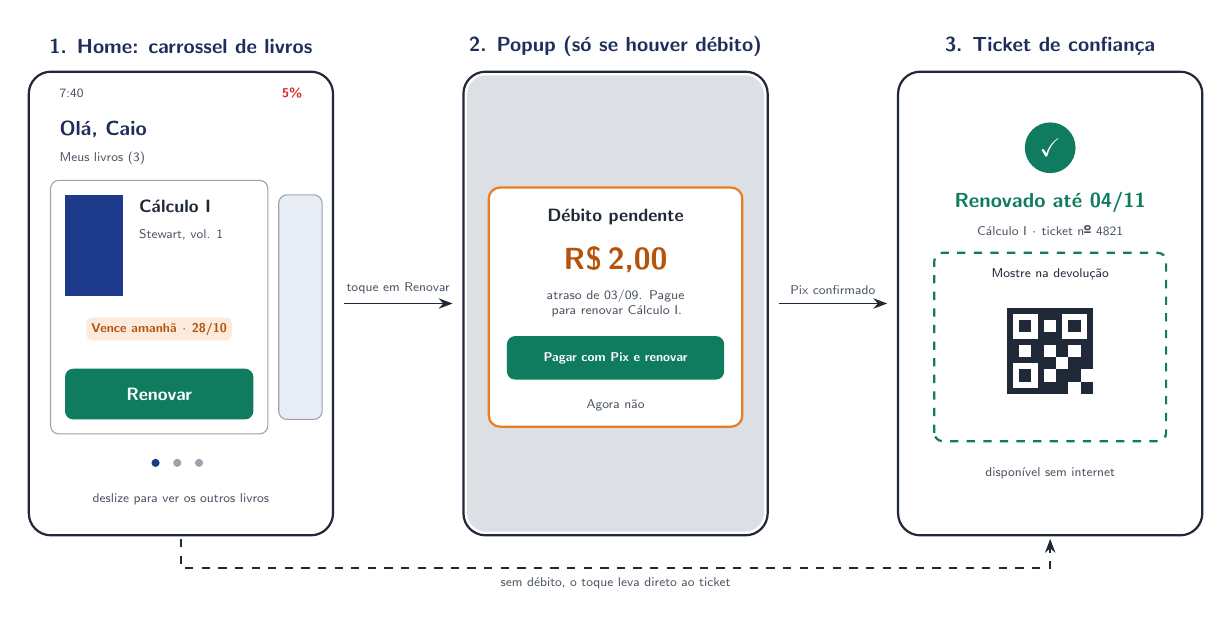
\begin{tikzpicture}[scale=0.92,transform shape,
  tela/.style={draw=labeltext,fill=white,rounded corners=8pt,line width=0.8pt},
  btn/.style={fill=verde,rounded corners=3pt},
  rot/.style={font=\footnotesize\bfseries,text=navytext},
  seta/.style={->,>={Stealth[length=5pt]},draw=labeltext,line width=0.6pt}]
  % ---------- Tela 1: home com carrossel ----------
  \draw[tela] (0,0) rectangle (4.2,6.4);
  \node[rot] at (2.1,6.75) {1. Home: carrossel de livros};
  \node[anchor=west,font=\tiny,text=subtle] at (0.3,6.1) {7:40};
  \node[anchor=east,font=\tiny\bfseries,text=dor] at (3.9,6.1) {5\%};
  \node[anchor=west,font=\footnotesize\bfseries,text=navytext] at (0.3,5.6) {Olá, Caio};
  \node[anchor=west,font=\tiny,text=subtle] at (0.3,5.2) {Meus livros (3)};
  \draw[gridline,fill=white,rounded corners=3pt] (0.3,1.4) rectangle (3.3,4.9);
  \fill[navy] (0.5,3.3) rectangle (1.3,4.7);
  \node[anchor=north west,font=\scriptsize\bfseries,text=labeltext] at (1.4,4.75) {Cálculo I};
  \node[anchor=north west,font=\tiny,text=subtle] at (1.4,4.35) {Stewart, vol. 1};
  \node[fill=laranjabg,text=amber,font=\tiny\bfseries,rounded corners=2pt,inner sep=2pt] at (1.8,2.85) {Vence amanhã $\cdot$ 28/10};
  \fill[btn] (0.5,1.6) rectangle (3.1,2.3);
  \node[font=\scriptsize\bfseries,text=white] at (1.8,1.95) {Renovar};
  \draw[gridline,fill=secbg,rounded corners=3pt] (3.45,1.6) rectangle (4.05,4.7);
  \fill[navy] (1.75,1.0) circle (1.6pt);
  \fill[gridline] (2.05,1.0) circle (1.6pt);
  \fill[gridline] (2.35,1.0) circle (1.6pt);
  \node[font=\tiny,text=subtle] at (2.1,0.5) {deslize para ver os outros livros};
  % ---------- Tela 2: popup de débito ----------
  \begin{scope}[xshift=6cm]
  \draw[tela] (0,0) rectangle (4.2,6.4);
  \fill[gridline!35,rounded corners=7pt] (0.05,0.05) rectangle (4.15,6.35);
  \node[rot] at (2.1,6.75) {2. Popup (só se houver débito)};
  \draw[laranja,fill=white,rounded corners=4pt,line width=0.8pt] (0.35,1.5) rectangle (3.85,4.8);
  \node[font=\scriptsize\bfseries,text=labeltext] at (2.1,4.4) {Débito pendente};
  \node[font=\large\bfseries,text=amber] at (2.1,3.8) {R\$\,2,00};
  \node[font=\tiny,text=subtle,text width=3cm,align=center] at (2.1,3.2) {atraso de 03/09. Pague para renovar Cálculo I.};
  \fill[btn] (0.6,2.15) rectangle (3.6,2.75);
  \node[font=\tiny\bfseries,text=white] at (2.1,2.45) {Pagar com Pix e renovar};
  \node[font=\tiny,text=subtle] at (2.1,1.8) {Agora não};
  \end{scope}
  % ---------- Tela 3: ticket de confiança ----------
  \begin{scope}[xshift=12cm]
  \draw[tela] (0,0) rectangle (4.2,6.4);
  \node[rot] at (2.1,6.75) {3. Ticket de confiança};
  \fill[verde] (2.1,5.35) circle (0.35);
  \node[text=white,font=\normalsize] at (2.1,5.35) {$\checkmark$};
  \node[font=\footnotesize\bfseries,text=verde] at (2.1,4.6) {Renovado até 04/11};
  \node[font=\tiny,text=subtle] at (2.1,4.2) {Cálculo I $\cdot$ ticket nº 4821};
  \draw[verde,dashed,rounded corners=3pt,line width=0.8pt] (0.5,1.3) rectangle (3.7,3.9);
  \node[font=\tiny,text=labeltext] at (2.1,3.6) {Mostre na devolução};
  \begin{scope}[shift={(1.5,1.95)},x=0.17cm,y=0.17cm]
    \foreach \a/\b in {0/4,4/4,0/0}{
      \fill[labeltext] (\a,\b) rectangle +(3,3);
      \fill[white] (\a+0.5,\b+0.5) rectangle +(2,2);
      \fill[labeltext] (\a+1,\b+1) rectangle +(1,1);}
    \foreach \a/\b in {3/0,4/1,6/0,5/2,6/2,3/2,4/3,6/3,0/3,2/3,3/4,3/6,4/0,5/1}{
      \fill[labeltext] (\a,\b) rectangle +(1,1);}
  \end{scope}
  \node[font=\tiny,text=subtle] at (2.1,0.85) {disponível sem internet};
  \end{scope}
  % setas entre as telas
  \draw[seta] (4.35,3.2) -- node[above,font=\tiny,text=subtle]{toque em Renovar} (5.85,3.2);
  \draw[seta] (10.35,3.2) -- node[above,font=\tiny,text=subtle]{Pix confirmado} (11.85,3.2);
  \draw[seta,dashed] (2.1,-0.05) -- (2.1,-0.45) -| node[pos=0.25,below,font=\tiny,text=subtle]{sem débito, o toque leva direto ao ticket} (14.1,-0.05);
\end{tikzpicture}
\end{caixa}

{\small
\textbf{Total de passos:} 4 (2 sem débito) \quad
\textbf{Decisões:} 2 \quad
\textbf{Ramos de erro:} 1 (com retorno) \quad
\textbf{O erro explica o que fazer?} $\boxtimes$ sim \ $\square$ não\par}
{\scriptsize\color{subtle}Antes: 6 passos e 3 decisões que o aluno precisava acompanhar. Agora: abrir o app e tocar em \textit{Renovar}; o popup só aparece quando há débito.\par}

\newpage
% =====================================================================
%  FOLHA 5 - REQUISITOS
% =====================================================================
\folha{Folha 5 -- Requisitos de design}{10 min}
\objetivo{Transformar pontos de dor e golfos em requisitos verificáveis e priorizados.}
\passos{(1) Pegue cada ponto de dor ou golfo. (2) Achado, insight, necessidade, requisito. (3) Torne verificável, com número ou teste. (4) Classifique o tipo. (5) Priorize: M (Must), S (Should), C (Could), W (Won't).}

{\footnotesize\renewcommand{\arraystretch}{1.3}%
\noindent
\begin{tabularx}{\linewidth}{|>{\raggedright\arraybackslash}p{2.45cm}|>{\raggedright\arraybackslash}p{2.45cm}|>{\raggedright\arraybackslash}p{2.3cm}|>{\raggedright\arraybackslash}X|>{\raggedright\arraybackslash}p{1.65cm}|>{\centering\arraybackslash}p{0.45cm}|}
\hline
\cab{secbg}{Achado} & \cab{secbg}{Insight} & \cab{laranjabg}{Necessidade} & \cab{verdebg}{Requisito (verificável)} & \cab{verdebg}{Tipo} & \cab{verdebg}{P} \\ \hline
\leavevmode\color{subtle}\scriptsize Ex.: botão cinza sem motivo & \leavevmode\color{subtle}\scriptsize Falta explicação & \leavevmode\color{subtle}\scriptsize Saber o motivo & \leavevmode\color{subtle}\scriptsize Explicar o bloqueio em até 1 toque & \leavevmode\color{subtle}\scriptsize usabilidade & \leavevmode\color{subtle}\scriptsize M \\ \hline
\textbf{R1.} Para renovar, Caio passa por várias telas e acha o botão cinza; nada avisa o prazo.\newline{\scriptsize\color{subtle}Origem: E1, E4, A3; dor 2.2}
& Cada tela a mais gasta bateria, sinal e paciência no ônibus.
& Renovar assim que abre o app, vendo o prazo de cada livro.
& A home mostra um \textbf{carrossel com um card por empréstimo} (capa, título, data e selo: ``Em dia'', ``Vence amanhã'' ou ``Débito pendente'') e um botão verde \textit{Renovar} de \textbf{no mínimo 48\,dp} na metade de baixo do card. Renovar exige \textbf{1 toque} a partir da home. Um aviso 48\,h antes do vencimento abre o app direto no card.\newline\textit{Teste:} 5 de 5 participantes renovam em \textbf{até 10\,s}, sem ajuda.
& Usabilidade & \bfseries M \\ \hline
\textbf{R2.} A multa só aparece na aba ``Débitos'' e o app não diz como pagar.\newline{\scriptsize\color{subtle}Origem: E2, E3, A4; dores 3.1 e 3.2}
& Caio não entende o bloqueio e a tarefa empaca.
& Resolver o débito sem sair da renovação.
& Com débito, o toque em \textit{Renovar} abre um \textbf{popup com o valor e o motivo em texto} e o botão ``Pagar com Pix e renovar''. Confirmado o Pix, a \textbf{renovação é feita automaticamente}, sem novo toque (\textbf{no máximo 2 toques} no total).\newline\textit{Teste:} funil popup $\rightarrow$ Pix $\rightarrow$ ticket; $\geq$ 70\% concluem em $\leq$ 2\,min.
& Usabilidade & \bfseries M \\ \hline
\textbf{R3.} Ao tocar em \textit{Renovar}, nada confirma a nova data.\newline{\scriptsize\color{subtle}Origem: A1; dor 4.2}
& Sem prova, Caio não confia e pode devolver atrasado.
& Ter certeza de que renovou e até quando.
& Em \textbf{até 2\,s} após a confirmação, o card vira um \textbf{ticket de confiança} com a nova data e um QR code, \textbf{visível sem internet}. Na devolução, a leitura do QR registra a entrega na hora e atualiza o ticket.\newline\textit{Teste:} 20 renovações em 3G simulado; todas mostram o ticket em $\leq$ 2\,s.
& Funcional & \bfseries M \\ \hline
\textbf{R4.} Com 3G instável, o pedido some sem aviso.\newline{\scriptsize\color{subtle}Origem: A2; dor 4.1}
& Caio repete toques e gasta bateria sem saber se deu certo.
& Não precisar acompanhar o pedido.
& O pedido (\textbf{no máximo 5\,KB}) entra numa fila e é \textbf{reenviado sozinho até 3 vezes}; o aluno vê só ``Renovando\ldots'' no card até o ticket aparecer. Toques repetidos \textbf{não geram pedido duplicado}.\newline\textit{Teste:} perfil ``Slow 3G'' com quedas de sinal.
& Não funcional (contexto) & \bfseries S \\ \hline
\end{tabularx}\par}
\vspace{4pt}
{\scriptsize\color{subtle}Tipos: funcional, não funcional, usabilidade, acessibilidade, contexto. Um bom requisito é necessário, claro, verificável, atômico e rastreável.\par}

\newpage
% =====================================================================
%  FOLHA 6 - HISTÓRIAS E CRITÉRIOS DE ACEITE
% =====================================================================
\folha{Folha 6 -- Histórias e critérios de aceite}{15 min}
\objetivo{Escrever histórias centradas na persona e critérios testáveis para as duas melhores.}
\passos{(1) Em silêncio, 5 min: 3 histórias por pessoa nos post-its. (2) 3 min: agrupar e eliminar duplicadas. (3) 3 min: testar o ``para que''. (4) 4 min: Dado--Quando--Então para as 2 melhores.}

\newcommand{\historia}[4]{%
  \begin{caixa}{História #1}
  \textbf{Como} #2, \textbf{quero} #3, \textbf{para que} #4.
  \end{caixa}}
\historia{1 \normalfont(R1)}{calouro com livro vencendo}{renovar direto na tela inicial, com um toque no card do livro}{eu resolva no ônibus em poucos segundos, sem ir à biblioteca}
\historia{2 \normalfont(R2)}{aluno com débito pendente}{pagar o débito num popup e ter a renovação feita automaticamente}{eu não precise procurar outra aba nem tocar em \textit{Renovar} de novo}
\historia{3 \normalfont(R3)}{aluno que vai devolver o livro}{um ticket de confiança com a nova data e um QR code}{eu tenha certeza da renovação e devolva sem fila no balcão}
\historia{4 \normalfont(R4)}{aluno com sinal fraco}{que o app termine a renovação sozinho quando a rede voltar}{eu não precise repetir o pedido nem gastar bateria}

\begin{caixa}[laranja]{Critério de aceite da história 1 \normalfont(renovação em 1 toque)}
\textbf{Cenário: renovação sem pendências}\par
\gk{Dado que} Caio tem ``Cálculo I'' vencendo amanhã e nenhum débito\par
\gk{quando} ele toca no botão verde \textit{Renovar} no card da home\par
\gk{então} em até 2\,s o card vira o ticket ``Renovado até 04/11'', com QR code, disponível sem internet.\par\vspace{3pt}
\textbf{Cenário: o sinal cai durante a renovação}\par
\gk{Dado que} Caio tocou em \textit{Renovar} com o 3G instável \gk{quando} o servidor não responde \gk{então} o card mostra só ``Renovando\ldots'', o app reenvia sozinho quando o sinal voltar e o ticket aparece, sem pedido duplicado.
\end{caixa}

\begin{caixa}[laranja]{Critério de aceite da história 2 \normalfont(débito em popup)}
\textbf{Cenário: renovação com débito pendente}\par
\gk{Dado que} Caio tem uma multa de R\$\,2,00\par
\gk{quando} ele toca em \textit{Renovar} no card da home\par
\gk{então} abre um popup com o valor, o motivo e o botão ``Pagar com Pix e renovar'',\par
\gk{e} quando o Pix é confirmado o livro é renovado e o ticket aparece, sem novo toque.\par\vspace{3pt}
\textbf{Cenário: o Pix não é confirmado}\par
\gk{Dado que} Caio pagou pelo popup \gk{quando} o banco não confirma em 60\,s \gk{então} o popup mostra ``Pagamento não confirmado. Toque para tentar de novo.'' e o livro continua no card com o prazo atual.
\end{caixa}

{\footnotesize\renewcommand{\arraystretch}{1.2}%
\noindent
\begin{tabularx}{\linewidth}{|l|c|c|c|c|c|c|X|}
\hline
\rowcolor{secbg}\bfseries INVEST & \bfseries Independente & \bfseries Negociável & \bfseries Valiosa & \bfseries Estimável & \bfseries Pequena & \bfseries Testável & \bfseries Observação \\ \hline
H1 & $\checkmark$ & $\checkmark$ & $\checkmark$ & $\checkmark$ & $\checkmark$ & $\checkmark$ & -- \\ \hline
H2 & parcial & $\checkmark$ & $\checkmark$ & $\checkmark$ & parcial & $\checkmark$ & Depende da H1 (o card com \textit{Renovar}) e da integração com o Pix. \\ \hline
H3 & $\checkmark$ & $\checkmark$ & $\checkmark$ & $\checkmark$ & $\checkmark$ & $\checkmark$ & -- \\ \hline
H4 & $\checkmark$ & $\checkmark$ & $\checkmark$ & $\checkmark$ & $\checkmark$ & $\checkmark$ & -- \\ \hline
\end{tabularx}\par}

\newpage
% =====================================================================
%  FOLHA 7 - FEATURES E PRIORIZAÇÃO
% =====================================================================
\folha{Folha 7 -- Features e priorização}{15 min}
\objetivo{Gerar features ligadas ao objetivo do negócio e priorizá-las com foco na pessoa.}
\passos{(1) 1 min: objetivo no centro. (2) 5 min: uma feature por post-it. (3) 2 min: agrupar. (4) 5 min: RICE em 4 features. (5) 2 min: matriz valor $\times$ esforço, 3 votos cada.}
{\small\textbf{Objetivo:} Reduzir em 30\% as devoluções em atraso.\par}

\begin{caixa}{Features agrupadas (nome do grupo e features)}
\renewcommand{\arraystretch}{1.2}%
\begin{tabularx}{\linewidth}{@{}>{\bfseries\raggedright\leavevmode\color{navytext}}p{3.2cm}X@{}}
Renovar em 1 toque & \textbf{F1} Carrossel de empréstimos na home, com selo de prazo e botão verde \textit{Renovar} \textbullet\ \textbf{F5} Renovação automática opcional \\
Resolver débito & \textbf{F2} Popup de débito com Pix e renovação automática \textbullet\ \textbf{F7} Perguntas frequentes \\
Dar certeza & \textbf{F3} Ticket de confiança (nova data + QR, offline, usado na devolução) \textbullet\ \textbf{F4} Processamento em segundo plano (fila e reenvio) \\
Lembrar & \textbf{F6} Aviso 2 dias antes, abrindo direto no card \textbullet\ \textbf{F8} Widget dos prazos \textbullet\ \textbf{F9} Chatbot da biblioteca \\
\end{tabularx}
\end{caixa}

{\footnotesize\renewcommand{\arraystretch}{1.3}%
\noindent
\begin{tabularx}{\linewidth}{|X|c|c|c|c|c|>{\columncolor{verdebg}}c|}
\hline
\rowcolor{secbg}\bfseries Feature & \bfseries A (0--10) & \bfseries I (1--3) & \bfseries C (0--1) & \bfseries E (1--13) & \bfseries Conta: (A$\times$I$\times$C)/E & \bfseries RICE \\ \hline
\leavevmode\color{subtle}Ex.: aviso antes do vencimento & \color{subtle}9 & \color{subtle}2 & \color{subtle}0,9 & \color{subtle}2 & \color{subtle}(9$\times$2$\times$0,9)/2 & \color{subtle}8,1 \\ \hline
\textbf{F1} Carrossel na home com \textit{Renovar} & 9 & 3 & 0,8 & 3 & (9$\times$3$\times$0,8)/3 = 21,6/3 & \bfseries 7,2 \\ \hline
\textbf{F3} Ticket de confiança & 8 & 2 & 0,8 & 2 & (8$\times$2$\times$0,8)/2 = 12,8/2 & \bfseries 6,4 \\ \hline
\textbf{F2} Popup de débito com Pix & 4 & 3 & 0,9 & 5 & (4$\times$3$\times$0,9)/5 = 10,8/5 & \bfseries 2,16 \\ \hline
\textbf{F4} Processamento em segundo plano & 5 & 2 & 0,6 & 5 & (5$\times$2$\times$0,6)/5 = 6,0/5 & \bfseries 1,2 \\ \hline
\end{tabularx}\par}
{\scriptsize\color{subtle}RICE = (Alcance $\times$ Impacto $\times$ Confiança) / Esforço. Esforço na sequência de Fibonacci (1, 2, 3, 5, 8, 13). \textbf{Por quê:} F1 atinge quase todo aluno com empréstimo (A\,=\,9) e reduz a renovação a 1 toque (I\,=\,3). F2 atinge só quem tem débito (A\,=\,4) e exige integrar o Pix (E\,=\,5). F4 tem confiança menor (C\,=\,0,6) porque ainda não sabemos quantos atrasos vêm de falha de rede.\par}

\vspace{8pt}
\noindent
\begin{minipage}[t]{0.5\linewidth}
\vspace{0pt}
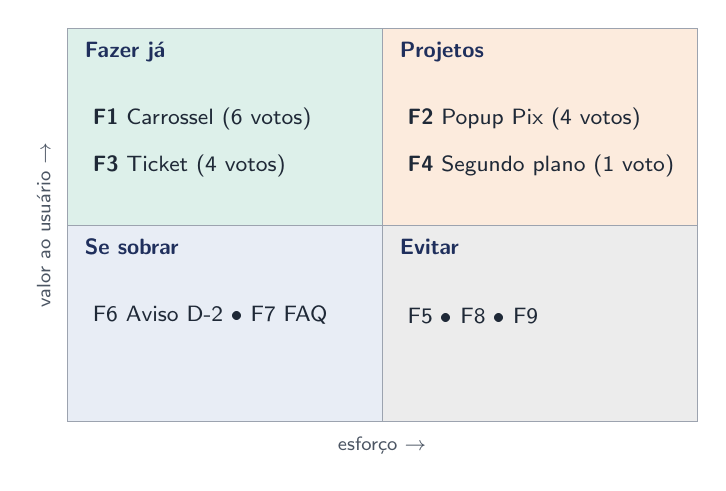
\begin{tikzpicture}[x=1cm,y=1cm,
  item/.style={anchor=west,font=\footnotesize,text=labeltext},
  quad/.style={anchor=north west,font=\footnotesize\bfseries,text=navytext}]
  \fill[verdebg] (0,2.5) rectangle (4,5);
  \fill[laranjabg] (4,2.5) rectangle (8,5);
  \fill[secbg] (0,0) rectangle (4,2.5);
  \fill[cinzabg] (4,0) rectangle (8,2.5);
  \draw[gridline] (0,0) rectangle (8,5); \draw[gridline] (4,0)--(4,5); \draw[gridline] (0,2.5)--(8,2.5);
  \node[quad] at (0.1,4.95) {Fazer já};
  \node[quad] at (4.1,4.95) {Projetos};
  \node[quad] at (0.1,2.45) {Se sobrar};
  \node[quad] at (4.1,2.45) {Evitar};
  \node[item] at (0.2,3.85) {\textbf{F1} Carrossel \hfill (6 votos)};
  \node[item] at (0.2,3.25) {\textbf{F3} Ticket \hfill (4 votos)};
  \node[item] at (4.2,3.85) {\textbf{F2} Popup Pix (4 votos)};
  \node[item] at (4.2,3.25) {\textbf{F4} Segundo plano (1 voto)};
  \node[item] at (0.2,1.35) {F6 Aviso D-2 \textbullet\ F7 FAQ};
  \node[item] at (4.2,1.35) {F5 \textbullet\ F8 \textbullet\ F9};
  \node[rotate=90,font=\scriptsize,text=subtle] at (-0.3,2.5) {valor ao usuário $\rightarrow$};
  \node[font=\scriptsize,text=subtle] at (4,-0.3) {esforço $\rightarrow$};
\end{tikzpicture}
\end{minipage}%
\hfill
\begin{minipage}[t]{0.46\linewidth}
\vspace{0pt}\small
\textbf{Como usamos:} post-its colados na matriz por consenso; cada pessoa votou com 3 pontos (15 votos).\par\vspace{5pt}
\textbf{Escopo da próxima entrega (features escolhidas):}
\begin{enumerate}[leftmargin=1.4em,itemsep=2pt]
  \item \textbf{F1} Carrossel com \textit{Renovar}: maior RICE (7,2) e mais votos.
  \item \textbf{F3} Ticket de confiança: RICE 6,4 e pouco esforço.
  \item \textbf{F2} Popup de débito com Pix: RICE menor (2,16), mas entra por cumprir R2 (Must). Sem ela, Caio continua travado.
\end{enumerate}
\vspace{3pt}
{\footnotesize\color{subtle}F4 roda no back-end junto com F1; a versão completa fica para a entrega seguinte.\par}
\end{minipage}

\newpage
% =====================================================================
%  FOLHA 8 - UX CANVAS E PITCH
% =====================================================================
\folha{Folha 8 -- UX Canvas e pitch}{15 min}
\objetivo{Reunir tudo em uma folha única e apresentar em 2 minutos.}
\passos{(1) 8 min: preencha as caixas na ordem 1 a 8. (2) 4 min: ensaie o pitch. (3) 3 min: apresente a outra equipe e anote um comentário.}

\newtcolorbox{canvas}[3]{enhanced,colback=white,colframe=#1,colbacktitle=#1,coltitle=white,
  fonttitle=\bfseries\small,halign title=center,title={#2},boxrule=0.6pt,arc=2pt,
  left=3pt,right=3pt,top=2pt,bottom=2pt,fontupper=\footnotesize\color{bodytext},
  before upper={{\color{subtle}\itshape #3}\par\vspace{2pt}}}

\begin{tcbraster}[raster columns=4,raster equal height=rows,raster column skip=4pt,raster row skip=5pt]
\begin{canvas}{navy}{1. Problema}{Qual dor resolver?}
Renovar pelo app exige várias telas, o bloqueio por débito não é explicado e nada confirma a nova data.
\end{canvas}
\begin{canvas}{navy}{2. Resultados}{O que o negócio ganha?}
$-30\%$ de devoluções em atraso e menos fila no balcão.
\end{canvas}
\begin{canvas}{verde}{3. Usuários}{Para quem?}
Alunos que usam o celular em trânsito, com pouca bateria e sinal fraco (Caio).
\end{canvas}
\begin{canvas}{verde}{4. Benefícios}{O que a pessoa ganha?}
Renovar em 1 toque na home, com certeza da nova data.
\end{canvas}
\begin{canvas}{laranja}{5. Ideias}{Que soluções?}
F1 carrossel com \textit{Renovar} \textbullet\ F2 popup de débito com Pix \textbullet\ F3 ticket de confiança.
\end{canvas}
\begin{canvas}{laranja}{6. Hipóteses}{Se fizermos X, então Y}
Se renovar for 1 toque na home, então os atrasos cairão $\geq$ 20\%.
\end{canvas}
\begin{canvas}{navy}{7. Aprender}{O que descobrir antes?}
Quais as causas dos atrasos? A universidade aceita Pix no app?
\end{canvas}
\begin{canvas}{navy}{8. Experimentos}{Como testar rápido?}
Protótipo com 5 calouros em 3G lento e teste A/B por 8 semanas.
\end{canvas}
\end{tcbraster}

\begin{caixa}{Roteiro do pitch (2 minutos)}
\renewcommand{\arraystretch}{1.35}%
\begin{tabularx}{\linewidth}{@{}>{\bfseries\raggedright\leavevmode\color{navy}\footnotesize}p{3.2cm}X@{}}
1. Persona e problema & Caio, no ônibus com 5\% de bateria, não consegue renovar o livro de Cálculo, que vence amanhã. \\
2. Golfos & Botão cinza sem motivo e débito escondido em outra aba (execução); nada confirma a nova data (avaliação). \\
3. Requisitos & Renovar em 1 toque na home (R1), débito em popup com Pix (R2) e ticket de confiança (R3). \\
4. Features & F1 carrossel (RICE 7,2) e F3 ticket (6,4) primeiro; F2 popup com Pix entra por ser Must. \\
5. Teste & Protótipo com 5 calouros em 3G lento e A/B por 8 semanas; meta de $\geq$ 20\% menos atrasos. \\
\end{tabularx}
\end{caixa}

\begin{caixa}{Comentário recebido da outra equipe}
\vspace{1.4cm}
\end{caixa}

\end{document}
